% Created by tikzDevice version 0.7.0 on 2014-10-06 20:08:18
% !TEX encoding = UTF-8 Unicode
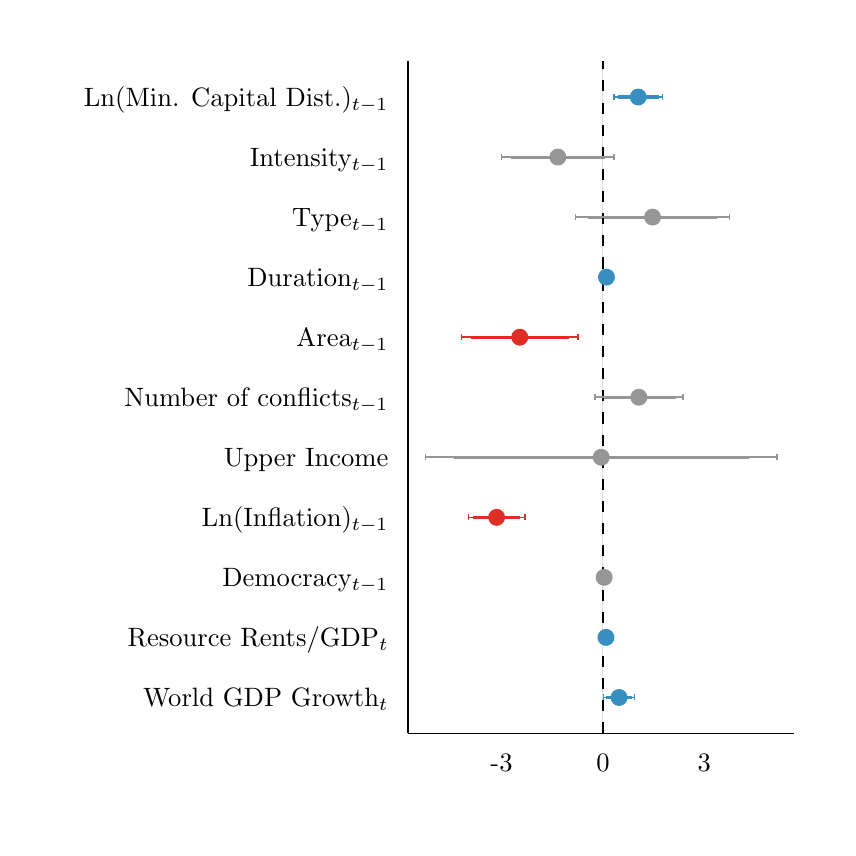
\begin{tikzpicture}[x=1pt,y=1pt]
\definecolor[named]{fillColor}{rgb}{1.00,1.00,1.00}
\path[use as bounding box,fill=fillColor,fill opacity=0.00] (0,0) rectangle (289.08,289.08);
\begin{scope}
\path[clip] (  0.00,  0.00) rectangle (289.08,289.08);
\definecolor[named]{drawColor}{rgb}{1.00,1.00,1.00}
\definecolor[named]{fillColor}{rgb}{1.00,1.00,1.00}

\path[draw=drawColor,line width= 0.6pt,line join=round,line cap=round,fill=fillColor] ( -0.00,  0.00) rectangle (289.08,289.08);
\end{scope}
\begin{scope}
\path[clip] (137.46, 34.03) rectangle (277.03,277.03);
\definecolor[named]{fillColor}{rgb}{1.00,1.00,1.00}

\path[fill=fillColor] (137.46, 34.03) rectangle (277.03,277.03);
\definecolor[named]{drawColor}{rgb}{0.21,0.56,0.75}
\definecolor[named]{fillColor}{rgb}{0.21,0.56,0.75}

\path[draw=drawColor,draw opacity=0.30,line width= 0.3pt,line join=round,fill=fillColor,fill opacity=0.30] (208.13, 47.05) -- (219.24, 47.05);

\path[draw=drawColor,draw opacity=0.30,line width= 0.3pt,line join=round,fill=fillColor,fill opacity=0.30] (208.14, 68.75) -- (209.77, 68.75);
\definecolor[named]{drawColor}{rgb}{0.59,0.59,0.59}
\definecolor[named]{fillColor}{rgb}{0.59,0.59,0.59}

\path[draw=drawColor,draw opacity=0.30,line width= 0.3pt,line join=round,fill=fillColor,fill opacity=0.30] (206.20, 90.45) -- (210.40, 90.45);
\definecolor[named]{drawColor}{rgb}{0.87,0.18,0.15}
\definecolor[named]{fillColor}{rgb}{0.87,0.18,0.15}

\path[draw=drawColor,draw opacity=0.30,line width= 0.3pt,line join=round,fill=fillColor,fill opacity=0.30] (159.27,112.14) -- (179.64,112.14);
\definecolor[named]{drawColor}{rgb}{0.59,0.59,0.59}
\definecolor[named]{fillColor}{rgb}{0.59,0.59,0.59}

\path[draw=drawColor,draw opacity=0.30,line width= 0.3pt,line join=round,fill=fillColor,fill opacity=0.30] (143.80,133.84) -- (270.69,133.84);

\path[draw=drawColor,draw opacity=0.30,line width= 0.3pt,line join=round,fill=fillColor,fill opacity=0.30] (205.01,155.53) -- (236.69,155.53);
\definecolor[named]{drawColor}{rgb}{0.87,0.18,0.15}
\definecolor[named]{fillColor}{rgb}{0.87,0.18,0.15}

\path[draw=drawColor,draw opacity=0.30,line width= 0.3pt,line join=round,fill=fillColor,fill opacity=0.30] (156.71,177.23) -- (198.91,177.23);
\definecolor[named]{drawColor}{rgb}{0.21,0.56,0.75}
\definecolor[named]{fillColor}{rgb}{0.21,0.56,0.75}

\path[draw=drawColor,draw opacity=0.30,line width= 0.3pt,line join=round,fill=fillColor,fill opacity=0.30] (208.28,198.93) -- (210.01,198.93);
\definecolor[named]{drawColor}{rgb}{0.59,0.59,0.59}
\definecolor[named]{fillColor}{rgb}{0.59,0.59,0.59}

\path[draw=drawColor,draw opacity=0.30,line width= 0.3pt,line join=round,fill=fillColor,fill opacity=0.30] (197.99,220.62) -- (253.62,220.62);

\path[draw=drawColor,draw opacity=0.30,line width= 0.3pt,line join=round,fill=fillColor,fill opacity=0.30] (171.25,242.32) -- (211.92,242.32);
\definecolor[named]{drawColor}{rgb}{0.21,0.56,0.75}
\definecolor[named]{fillColor}{rgb}{0.21,0.56,0.75}

\path[draw=drawColor,draw opacity=0.30,line width= 0.3pt,line join=round,fill=fillColor,fill opacity=0.30] (211.83,264.02) -- (229.44,264.02);
\definecolor[named]{drawColor}{rgb}{0.21,0.56,0.75}
\definecolor[named]{fillColor}{rgb}{0.21,0.56,0.75}

\path[draw=drawColor,line width= 1.1pt,line join=round,fill=fillColor] (209.03, 47.05) -- (218.35, 47.05);

\path[draw=drawColor,line width= 1.1pt,line join=round,fill=fillColor] (208.27, 68.75) -- (209.64, 68.75);
\definecolor[named]{drawColor}{rgb}{0.59,0.59,0.59}
\definecolor[named]{fillColor}{rgb}{0.59,0.59,0.59}

\path[draw=drawColor,line width= 1.1pt,line join=round,fill=fillColor] (206.54, 90.45) -- (210.06, 90.45);
\definecolor[named]{drawColor}{rgb}{0.87,0.18,0.15}
\definecolor[named]{fillColor}{rgb}{0.87,0.18,0.15}

\path[draw=drawColor,line width= 1.1pt,line join=round,fill=fillColor] (160.90,112.14) -- (178.00,112.14);
\definecolor[named]{drawColor}{rgb}{0.59,0.59,0.59}
\definecolor[named]{fillColor}{rgb}{0.59,0.59,0.59}

\path[draw=drawColor,line width= 1.1pt,line join=round,fill=fillColor] (154.00,133.84) -- (260.49,133.84);

\path[draw=drawColor,line width= 1.1pt,line join=round,fill=fillColor] (207.55,155.53) -- (234.14,155.53);
\definecolor[named]{drawColor}{rgb}{0.87,0.18,0.15}
\definecolor[named]{fillColor}{rgb}{0.87,0.18,0.15}

\path[draw=drawColor,line width= 1.1pt,line join=round,fill=fillColor] (160.10,177.23) -- (195.52,177.23);
\definecolor[named]{drawColor}{rgb}{0.21,0.56,0.75}
\definecolor[named]{fillColor}{rgb}{0.21,0.56,0.75}

\path[draw=drawColor,line width= 1.1pt,line join=round,fill=fillColor] (208.42,198.93) -- (209.87,198.93);
\definecolor[named]{drawColor}{rgb}{0.59,0.59,0.59}
\definecolor[named]{fillColor}{rgb}{0.59,0.59,0.59}

\path[draw=drawColor,line width= 1.1pt,line join=round,fill=fillColor] (202.46,220.62) -- (249.15,220.62);

\path[draw=drawColor,line width= 1.1pt,line join=round,fill=fillColor] (174.52,242.32) -- (208.65,242.32);
\definecolor[named]{drawColor}{rgb}{0.21,0.56,0.75}
\definecolor[named]{fillColor}{rgb}{0.21,0.56,0.75}

\path[draw=drawColor,line width= 1.1pt,line join=round,fill=fillColor] (213.24,264.02) -- (228.03,264.02);
\definecolor[named]{drawColor}{rgb}{0.00,0.00,0.00}
\definecolor[named]{fillColor}{rgb}{0.00,0.00,0.00}

\path[draw=drawColor,line width= 0.6pt,dash pattern=on 4pt off 4pt ,line join=round,fill=fillColor] (207.86, 34.03) -- (207.86,277.03);
\definecolor[named]{drawColor}{rgb}{0.21,0.56,0.75}
\definecolor[named]{fillColor}{rgb}{0.21,0.56,0.75}

\path[draw=drawColor,line width= 0.4pt,line join=round,line cap=round,fill=fillColor] (220.63,264.02) circle (  2.85);
\definecolor[named]{drawColor}{rgb}{0.59,0.59,0.59}
\definecolor[named]{fillColor}{rgb}{0.59,0.59,0.59}

\path[draw=drawColor,line width= 0.4pt,line join=round,line cap=round,fill=fillColor] (191.58,242.32) circle (  2.85);

\path[draw=drawColor,line width= 0.4pt,line join=round,line cap=round,fill=fillColor] (225.80,220.62) circle (  2.85);
\definecolor[named]{drawColor}{rgb}{0.21,0.56,0.75}
\definecolor[named]{fillColor}{rgb}{0.21,0.56,0.75}

\path[draw=drawColor,line width= 0.4pt,line join=round,line cap=round,fill=fillColor] (209.15,198.93) circle (  2.85);
\definecolor[named]{drawColor}{rgb}{0.87,0.18,0.15}
\definecolor[named]{fillColor}{rgb}{0.87,0.18,0.15}

\path[draw=drawColor,line width= 0.4pt,line join=round,line cap=round,fill=fillColor] (177.81,177.23) circle (  2.85);
\definecolor[named]{drawColor}{rgb}{0.59,0.59,0.59}
\definecolor[named]{fillColor}{rgb}{0.59,0.59,0.59}

\path[draw=drawColor,line width= 0.4pt,line join=round,line cap=round,fill=fillColor] (220.85,155.53) circle (  2.85);

\path[draw=drawColor,line width= 0.4pt,line join=round,line cap=round,fill=fillColor] (207.25,133.84) circle (  2.85);
\definecolor[named]{drawColor}{rgb}{0.87,0.18,0.15}
\definecolor[named]{fillColor}{rgb}{0.87,0.18,0.15}

\path[draw=drawColor,line width= 0.4pt,line join=round,line cap=round,fill=fillColor] (169.45,112.14) circle (  2.85);
\definecolor[named]{drawColor}{rgb}{0.59,0.59,0.59}
\definecolor[named]{fillColor}{rgb}{0.59,0.59,0.59}

\path[draw=drawColor,line width= 0.4pt,line join=round,line cap=round,fill=fillColor] (208.30, 90.45) circle (  2.85);
\definecolor[named]{drawColor}{rgb}{0.21,0.56,0.75}
\definecolor[named]{fillColor}{rgb}{0.21,0.56,0.75}

\path[draw=drawColor,line width= 0.4pt,line join=round,line cap=round,fill=fillColor] (208.96, 68.75) circle (  2.85);

\path[draw=drawColor,line width= 0.4pt,line join=round,line cap=round,fill=fillColor] (213.69, 47.05) circle (  2.85);

\path[draw=drawColor,line width= 0.6pt,line join=round] (219.24, 45.97) --
	(219.24, 48.14);

\path[draw=drawColor,line width= 0.6pt,line join=round] (219.24, 47.05) --
	(208.13, 47.05);

\path[draw=drawColor,line width= 0.6pt,line join=round] (208.13, 45.97) --
	(208.13, 48.14);

\path[draw=drawColor,line width= 0.6pt,line join=round] (209.77, 67.66) --
	(209.77, 69.83);

\path[draw=drawColor,line width= 0.6pt,line join=round] (209.77, 68.75) --
	(208.14, 68.75);

\path[draw=drawColor,line width= 0.6pt,line join=round] (208.14, 67.66) --
	(208.14, 69.83);
\definecolor[named]{drawColor}{rgb}{0.59,0.59,0.59}

\path[draw=drawColor,line width= 0.6pt,line join=round] (210.40, 89.36) --
	(210.40, 91.53);

\path[draw=drawColor,line width= 0.6pt,line join=round] (210.40, 90.45) --
	(206.20, 90.45);

\path[draw=drawColor,line width= 0.6pt,line join=round] (206.20, 89.36) --
	(206.20, 91.53);
\definecolor[named]{drawColor}{rgb}{0.87,0.18,0.15}

\path[draw=drawColor,line width= 0.6pt,line join=round] (179.64,111.06) --
	(179.64,113.23);

\path[draw=drawColor,line width= 0.6pt,line join=round] (179.64,112.14) --
	(159.27,112.14);

\path[draw=drawColor,line width= 0.6pt,line join=round] (159.27,111.06) --
	(159.27,113.23);
\definecolor[named]{drawColor}{rgb}{0.59,0.59,0.59}

\path[draw=drawColor,line width= 0.6pt,line join=round] (270.69,132.75) --
	(270.69,134.92);

\path[draw=drawColor,line width= 0.6pt,line join=round] (270.69,133.84) --
	(143.80,133.84);

\path[draw=drawColor,line width= 0.6pt,line join=round] (143.80,132.75) --
	(143.80,134.92);

\path[draw=drawColor,line width= 0.6pt,line join=round] (236.69,154.45) --
	(236.69,156.62);

\path[draw=drawColor,line width= 0.6pt,line join=round] (236.69,155.53) --
	(205.01,155.53);

\path[draw=drawColor,line width= 0.6pt,line join=round] (205.01,154.45) --
	(205.01,156.62);
\definecolor[named]{drawColor}{rgb}{0.87,0.18,0.15}

\path[draw=drawColor,line width= 0.6pt,line join=round] (198.91,176.15) --
	(198.91,178.32);

\path[draw=drawColor,line width= 0.6pt,line join=round] (198.91,177.23) --
	(156.71,177.23);

\path[draw=drawColor,line width= 0.6pt,line join=round] (156.71,176.15) --
	(156.71,178.32);
\definecolor[named]{drawColor}{rgb}{0.21,0.56,0.75}

\path[draw=drawColor,line width= 0.6pt,line join=round] (210.01,197.84) --
	(210.01,200.01);

\path[draw=drawColor,line width= 0.6pt,line join=round] (210.01,198.93) --
	(208.28,198.93);

\path[draw=drawColor,line width= 0.6pt,line join=round] (208.28,197.84) --
	(208.28,200.01);
\definecolor[named]{drawColor}{rgb}{0.59,0.59,0.59}

\path[draw=drawColor,line width= 0.6pt,line join=round] (253.62,219.54) --
	(253.62,221.71);

\path[draw=drawColor,line width= 0.6pt,line join=round] (253.62,220.62) --
	(197.99,220.62);

\path[draw=drawColor,line width= 0.6pt,line join=round] (197.99,219.54) --
	(197.99,221.71);

\path[draw=drawColor,line width= 0.6pt,line join=round] (211.92,241.24) --
	(211.92,243.41);

\path[draw=drawColor,line width= 0.6pt,line join=round] (211.92,242.32) --
	(171.25,242.32);

\path[draw=drawColor,line width= 0.6pt,line join=round] (171.25,241.24) --
	(171.25,243.41);
\definecolor[named]{drawColor}{rgb}{0.21,0.56,0.75}

\path[draw=drawColor,line width= 0.6pt,line join=round] (229.44,262.93) --
	(229.44,265.10);

\path[draw=drawColor,line width= 0.6pt,line join=round] (229.44,264.02) --
	(211.83,264.02);

\path[draw=drawColor,line width= 0.6pt,line join=round] (211.83,262.93) --
	(211.83,265.10);
\end{scope}
\begin{scope}
\path[clip] (  0.00,  0.00) rectangle (289.08,289.08);
\definecolor[named]{drawColor}{rgb}{0.00,0.00,0.00}

\path[draw=drawColor,line width= 0.6pt,line join=round] (137.46, 34.03) --
	(137.46,277.03);
\end{scope}
\begin{scope}
\path[clip] (  0.00,  0.00) rectangle (289.08,289.08);
\definecolor[named]{drawColor}{rgb}{0.00,0.00,0.00}

\node[text=drawColor,anchor=base east,inner sep=0pt, outer sep=0pt, scale=  0.96] at (130.35, 43.75) {World GDP Growth$_{t}$};

\node[text=drawColor,anchor=base east,inner sep=0pt, outer sep=0pt, scale=  0.96] at (130.35, 65.44) {Resource Rents/GDP$_{t}$};

\node[text=drawColor,anchor=base east,inner sep=0pt, outer sep=0pt, scale=  0.96] at (130.35, 87.14) {Democracy$_{t-1}$};

\node[text=drawColor,anchor=base east,inner sep=0pt, outer sep=0pt, scale=  0.96] at (130.35,108.84) {Ln(Inflation)$_{t-1}$};

\node[text=drawColor,anchor=base east,inner sep=0pt, outer sep=0pt, scale=  0.96] at (130.35,130.53) {Upper Income};

\node[text=drawColor,anchor=base east,inner sep=0pt, outer sep=0pt, scale=  0.96] at (130.35,152.23) {Number of conflicts$_{t-1}$};

\node[text=drawColor,anchor=base east,inner sep=0pt, outer sep=0pt, scale=  0.96] at (130.35,173.93) {Area$_{t-1}$};

\node[text=drawColor,anchor=base east,inner sep=0pt, outer sep=0pt, scale=  0.96] at (130.35,195.62) {Duration$_{t-1}$};

\node[text=drawColor,anchor=base east,inner sep=0pt, outer sep=0pt, scale=  0.96] at (130.35,217.32) {Type$_{t-1}$};

\node[text=drawColor,anchor=base east,inner sep=0pt, outer sep=0pt, scale=  0.96] at (130.35,239.01) {Intensity$_{t-1}$};

\node[text=drawColor,anchor=base east,inner sep=0pt, outer sep=0pt, scale=  0.96] at (130.35,260.71) {Ln(Min. Capital Dist.)$_{t-1}$};
\end{scope}
\begin{scope}
\path[clip] (  0.00,  0.00) rectangle (289.08,289.08);
\definecolor[named]{drawColor}{rgb}{0.00,0.00,0.00}

\path[draw=drawColor,line width= 0.6pt,line join=round] (137.46, 34.03) --
	(277.03, 34.03);
\end{scope}
\begin{scope}
\path[clip] (  0.00,  0.00) rectangle (289.08,289.08);
\definecolor[named]{drawColor}{rgb}{0.00,0.00,0.00}

\node[text=drawColor,anchor=base,inner sep=0pt, outer sep=0pt, scale=  0.96] at (171.21, 20.31) {-3};

\node[text=drawColor,anchor=base,inner sep=0pt, outer sep=0pt, scale=  0.96] at (207.86, 20.31) {0};

\node[text=drawColor,anchor=base,inner sep=0pt, outer sep=0pt, scale=  0.96] at (244.52, 20.31) {3};
\end{scope}
\end{tikzpicture}
